% This file is part of GUFI, which is part of MarFS, which is released
% under the BSD license.
%
%
% Copyright (c) 2017, Los Alamos National Security (LANS), LLC
% All rights reserved.
%
% Redistribution and use in source and binary forms, with or without modification,
% are permitted provided that the following conditions are met:
%
% 1. Redistributions of source code must retain the above copyright notice, this
% list of conditions and the following disclaimer.
%
% 2. Redistributions in binary form must reproduce the above copyright notice,
% this list of conditions and the following disclaimer in the documentation and/or
% other materials provided with the distribution.
%
% 3. Neither the name of the copyright holder nor the names of its contributors
% may be used to endorse or promote products derived from this software without
% specific prior written permission.
%
% THIS SOFTWARE IS PROVIDED BY THE COPYRIGHT HOLDERS AND CONTRIBUTORS "AS IS" AND
% ANY EXPRESS OR IMPLIED WARRANTIES, INCLUDING, BUT NOT LIMITED TO, THE IMPLIED
% WARRANTIES OF MERCHANTABILITY AND FITNESS FOR A PARTICULAR PURPOSE ARE DISCLAIMED.
% IN NO EVENT SHALL THE COPYRIGHT HOLDER OR CONTRIBUTORS BE LIABLE FOR ANY DIRECT,
% INDIRECT, INCIDENTAL, SPECIAL, EXEMPLARY, OR CONSEQUENTIAL DAMAGES (INCLUDING,
% BUT NOT LIMITED TO, PROCUREMENT OF SUBSTITUTE GOODS OR SERVICES; LOSS OF USE,
% DATA, OR PROFITS; OR BUSINESS INTERRUPTION) HOWEVER CAUSED AND ON ANY THEORY OF
% LIABILITY, WHETHER IN CONTRACT, STRICT LIABILITY, OR TORT (INCLUDING NEGLIGENCE
% OR OTHERWISE) ARISING IN ANY WAY OUT OF THE USE OF THIS SOFTWARE, EVEN IF
% ADVISED OF THE POSSIBILITY OF SUCH DAMAGE.
%
%
% From Los Alamos National Security, LLC:
% LA-CC-15-039
%
% Copyright (c) 2017, Los Alamos National Security, LLC All rights reserved.
% Copyright 2017. Los Alamos National Security, LLC. This software was produced
% under U.S. Government contract DE-AC52-06NA25396 for Los Alamos National
% Laboratory (LANL), which is operated by Los Alamos National Security, LLC for
% the U.S. Department of Energy. The U.S. Government has rights to use,
% reproduce, and distribute this software.  NEITHER THE GOVERNMENT NOR LOS
% ALAMOS NATIONAL SECURITY, LLC MAKES ANY WARRANTY, EXPRESS OR IMPLIED, OR
% ASSUMES ANY LIABILITY FOR THE USE OF THIS SOFTWARE.  If software is
% modified to produce derivative works, such modified software should be
% clearly marked, so as not to confuse it with the version available from
% LANL.
%
% THIS SOFTWARE IS PROVIDED BY LOS ALAMOS NATIONAL SECURITY, LLC AND CONTRIBUTORS
% "AS IS" AND ANY EXPRESS OR IMPLIED WARRANTIES, INCLUDING, BUT NOT LIMITED TO,
% THE IMPLIED WARRANTIES OF MERCHANTABILITY AND FITNESS FOR A PARTICULAR PURPOSE
% ARE DISCLAIMED. IN NO EVENT SHALL LOS ALAMOS NATIONAL SECURITY, LLC OR
% CONTRIBUTORS BE LIABLE FOR ANY DIRECT, INDIRECT, INCIDENTAL, SPECIAL,
% EXEMPLARY, OR CONSEQUENTIAL DAMAGES (INCLUDING, BUT NOT LIMITED TO, PROCUREMENT
% OF SUBSTITUTE GOODS OR SERVICES; LOSS OF USE, DATA, OR PROFITS; OR BUSINESS
% INTERRUPTION) HOWEVER CAUSED AND ON ANY THEORY OF LIABILITY, WHETHER IN
% CONTRACT, STRICT LIABILITY, OR TORT (INCLUDING NEGLIGENCE OR OTHERWISE) ARISING
% IN ANY WAY OUT OF THE USE OF THIS SOFTWARE, EVEN IF ADVISED OF THE POSSIBILITY
% OF SUCH DAMAGE.


\section{Understanding the data and how its stored}
The data stored in these databases include filenames, access and creation dates, file attributes, and extended attributes. At the time of creating this document; depending on which table is viewed and what view is selected, there are currently 59 possible attributes(columns) per entry(row). More attributes may be added in the future. 
\\
\\
\subsection{Tables}
The \textbf{entries table} houses extracted metadata for files and links within the corresponding directory.  Database rows capture file name, size, inode (primary key), These are vital facts (attributes and extended attributes) about files without the heft of the actual files.
\\
\\
 The directory \textbf{summary table} houses extracted information about everything within the corresponding directory. It is a summary of that directory, including information about minimum file size, maximum file size, the number of files, and more. 
\\
\\
\begin{figure} [h]
\centering
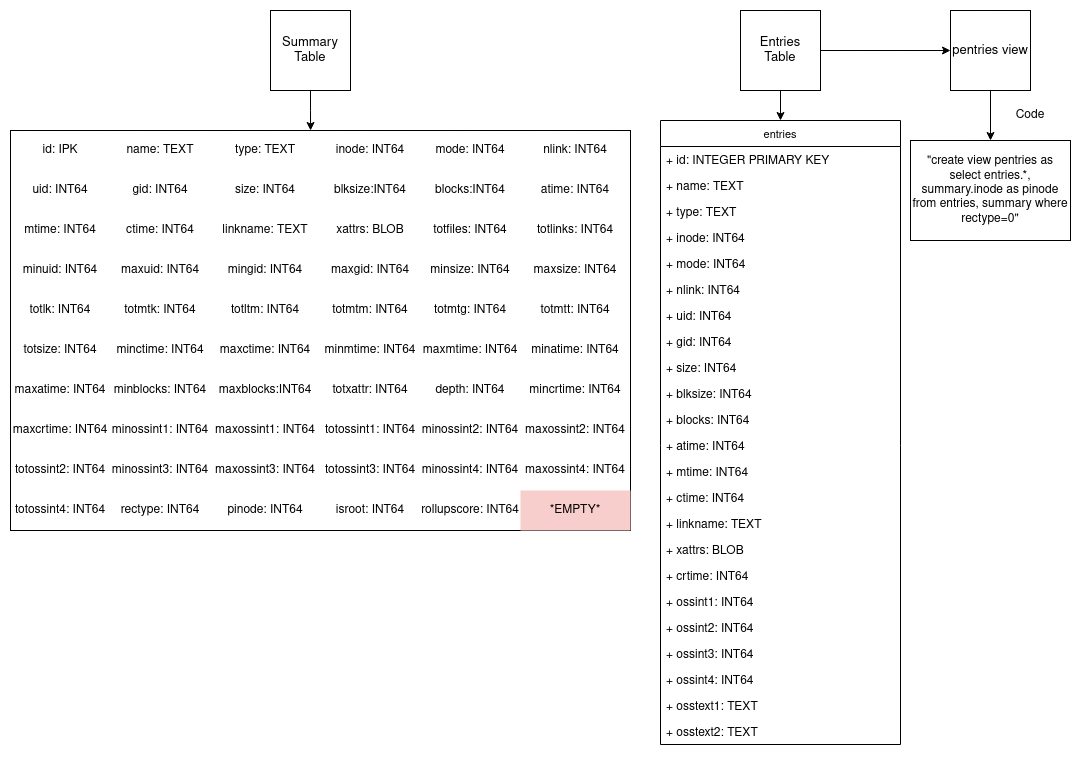
\includegraphics[width=1.0\textwidth]{images/Database_Schemas.png}
\caption{\label{fig:Database Schema}Database schema}
\end{figure}

\subsection{pentries view}
\begin{itemize}
  \item Provides parent inode as a query-able variable to the entries table
  \item Exists solely because parent inodes are not stored
  \item Parent inode is calculated/looked up so that parent inodes are never stored with child records.
\end{itemize}